% LNCS only: no article fallback; retain publisher typography and page geometry.
\newif\iflncsformat
\lncsformattrue
\documentclass[runningheads]{llncs}
\usepackage{amsmath,amssymb,booktabs,array,url,graphicx}
\usepackage{placeins}
\usepackage{flafter}
\setcounter{topnumber}{3}
\setcounter{bottomnumber}{2}
\setcounter{totalnumber}{5}
\renewcommand{\topfraction}{0.9}
\renewcommand{\bottomfraction}{0.8}
\renewcommand{\textfraction}{0.1}
\renewcommand{\floatpagefraction}{0.75}
\usepackage{xcolor}
\usepackage{tikz}
\usetikzlibrary{arrows.meta,positioning}
\usepackage{algorithm}
\usepackage{algpseudocode}
\definecolor{RevisionBlue}{RGB}{0,70,175}
% Set to false for a clean manuscript; blue marks revised/new text.
\newif\ifmarkrevisions
\markrevisionstrue
\newcommand{\rev}[1]{\ifmarkrevisions{\color{RevisionBlue}#1}\else#1\fi}
\newenvironment{revision}{\par\begingroup\ifmarkrevisions\color{RevisionBlue}\fi}{\par\endgroup}
\usepackage{microtype} % 微观排版优化，自然紧凑行数

% Retain LNCS typography; modest spacing without shrinking body text.
\setlength{\abovedisplayskip}{6pt plus 1pt minus 1pt}
\setlength{\belowdisplayskip}{6pt plus 1pt minus 1pt}
\setlength{\textfloatsep}{10pt plus 2pt minus 2pt}
\setlength{\intextsep}{8pt plus 2pt minus 2pt}
\setlength{\abovecaptionskip}{5pt plus 1pt minus 1pt}

% Figure filenames are unchanged. Search order:
% figures/<name>.pdf, <name>.pdf, figures/<name>.png, <name>.png.
\newif\ifshowfigures
\showfigurestrue
\newcommand{\figurebox}[2]{%
  \fbox{\parbox[c][#2][c]{0.92\linewidth}{\centering
  Figure reserved\\[3pt]\small\texttt{\detokenize{#1}}}}}
\newcommand{\paperfigure}[2]{%
  \ifshowfigures
    \IfFileExists{figures/#1.pdf}{%
      \includegraphics[width=\linewidth]{figures/#1.pdf}%
    }{\IfFileExists{#1.pdf}{%
      \includegraphics[width=\linewidth]{#1.pdf}%
    }{\IfFileExists{figures/#1.png}{%
      \includegraphics[width=\linewidth]{figures/#1.png}%
    }{\IfFileExists{#1.png}{%
      \includegraphics[width=\linewidth]{#1.png}%
    }{%
      \PackageWarning{paperfigures}{Missing figure: #1 (PDF/PNG in figures/ or project root)}%
      \figurebox{#1}{#2}%
    }}}}%
  \else\figurebox{#1}{#2}\fi}
\iflncsformat\else
\usepackage[margin=26mm]{geometry}
\fi
\usepackage[hidelinks]{hyperref}
\usepackage{refcount}
\AtEndDocument{%
  \ifnum\getpagerefnumber{page:referencesstart}=0
    \PackageWarningNoLine{pagebudget}{Rerun LaTeX to check the 12-page body limit}%
  \else
    \typeout{PAPER-BODY-PAGES: \number\numexpr\getpagerefnumber{page:referencesstart}-1\relax}%
    \ifnum\getpagerefnumber{page:referencesstart}>13
      \PackageWarningNoLine{pagebudget}{Body exceeds 12 pages; revise before submission}%
    \fi
  \fi}
\newcommand{\EII}{\textsc{EII}}
\newcommand{\PT}{\textsc{PerTarget}}
\newcommand{\CU}{\textsc{CachedUnion}}
\newcommand{\FT}{\textsc{FullTree}}
\newcommand{\CP}{\textsc{CostPlanner}}
\newcommand{\PolicyState}{\mathcal S}
\newcommand{\Result}{\mathsf{Result}}
\newcommand{\Witness}{\mathsf{Witness}}
\newcommand{\Eval}{\mathsf{Eval}}
\newcommand{\Finalize}{\mathsf{Finalize}}
\newcommand{\Key}{\mathsf{Key}}
\setlength{\emergencystretch}{2em}

\title{\rev{Shared-Witness Authorization for Multi-File Queries over Revocable Hierarchical Encrypted Data}}
\iflncsformat
\titlerunning{Shared-Witness Multi-File Authorization}
\author{Xinlin Gao\inst{1} \and Chungen Xu\inst{2}\thanks{Corresponding author.} \and Gangyi Chen\inst{1}}
\authorrunning{X. Gao et al.}

\institute{
School of Cyber Science and Engineering,
Nanjing University of Science and Technology,
Nanjing 210094, China\\
\email{gaoxinlin@njust.edu.cn, 324127010356@njust.edu.cn}
\and
School of Mathematics and Statistics,
Nanjing University of Science and Technology,
Nanjing 210094, China\\
\email{xuchung@njust.edu.cn}
}
\fi

\begin{document}
\maketitle
\begin{abstract}
\begin{revision}
Encrypted cloud storage must support file retrieval and access control
while protecting data privacy. When a single user's query returns multiple
files, authorization is typically performed separately for each candidate.
If their hierarchical access policies overlap, this can repeat the same
cryptographic computations. We propose Cached-UnionWitness, a shared-witness
authorization method that combines the satisfying witnesses of candidate
files and reuses identical leaf transformations and intermediate
reconstruction results. We analyze the conditions under which reuse preserves
authorization results and evaluate the method through correctness tests,
ablation experiments, and an independent holdout. For 16 same-branch
candidates, shared-witness execution reduces authorization time by about
14\% relative to per-target authorization with the same attribute-header
cache, with the benefit reproduced in the holdout. The results further show
that the gains vary with witness overlap, providing an execution method for
reducing repeated cryptographic work in multi-file authorization over
hierarchical encrypted data.
\end{revision}

\iflncsformat
\keywords{\rev{Encrypted cloud storage \and Hierarchical access control \and Attribute-based encryption \and Witness reuse \and Batch authorization}}
\fi
\end{abstract}

\section{Introduction}
\begin{revision}
Cloud storage must protect uploaded files while allowing users to find and
access them. Searchable encryption supports retrieval over encrypted
data~\cite{Song2000EncryptedSearch,Curtmola2006SSE}, while attribute-based
encryption controls decryption through roles, departments, and other
attributes~\cite{Bethencourt2007CPABE,Waters2011CPABE}. A query returning
multiple files therefore requires both retrieval and authorization. We
address the latter stage, where independent processing may repeat expensive
cryptographic work.

This repetition arises when files share a hierarchical authorization tree.
Files occupy internal nodes, and each file's policy is its rooted subtree.
A project query may return a summary and a subordinate report: if the
summary's selected authorization path includes the report's subtree, both
require the same leaf transformations and intermediate reconstructions.
Figure~\ref{fig:worked} illustrates five leaf evaluations reducible to three.
The opportunity depends on the selected policies, not directory proximity.

Matching attribute names or policy shapes is insufficient because equally
labeled leaves may contain different encrypted shares. Cached-UnionWitness
instead selects a satisfying witness for each candidate and merges operations
only when their cryptographic inputs and authorization state match. It
evaluates shared leaves and reconstructions once, retaining each file's final
transform and user recovery. The CSP performs both retrieval and authorization
(Fig.~\ref{fig:system}); reuse concerns one user's query on a fixed ciphertext
snapshot, with concurrent updates requiring snapshot pinning or retry.

We establish conditional result preservation and separate witness sharing
from attribute-header caching through a four-way ablation. For 16 same-branch
candidates, median authorization speedups over equally cached per-target
execution are $1.163\times$ in discovery and $1.159\times$ in a fresh-seed
holdout. Revocation and controlled complete-call experiments measure the
surrounding costs.
\end{revision}

\section{Related Work}
\begin{revision}
\paragraph{Encrypted retrieval and access control.}
Searchable encryption supports encrypted lookup and Boolean
queries~\cite{Song2000EncryptedSearch,Curtmola2006SSE,Cash2013BooleanSSE};
hierarchical and revocable attribute-based keyword search also enforce
policies~\cite{Miao2020ABKSHD,Cui2018AKSER}. These schemes supply candidates,
but do not resolve our post-retrieval execution question: which candidate
authorizations can share computations? Search-update
privacy~\cite{Bost2017ForwardBackward} concerns index leakage rather than
attribute revocation.

\paragraph{Hierarchical and outsourced encryption.}
Ciphertext-policy ABE expresses decryption
conditions~\cite{Bethencourt2007CPABE,Waters2011CPABE}, and file-hierarchy ABE
organizes layered policies~\cite{Wang2016FileHierarchy}. Outsourcing moves
transforms to a server, with verifiable variants checking
results~\cite{Green2011OutsourcedABE,Lai2013Verifiable}; fast-decryption
schemes change the construction to reduce
pairings~\cite{Hohenberger2013Fast}. Building on file-hierarchy CP-ABE, we
incorporate attribute revocation without updating users' existing secret
keys, using attribute-revocation and user-cover
techniques~\cite{Yu2010AttributeRevocation,Naor2001Cover}, and optimize
multi-file authorization through shared-witness execution. Revocation
updates ciphertexts and attribute headers rather than user secret keys.

\paragraph{Batching and shared execution.}
Portunus studies distributed ABE access control~\cite{Ladd2023Portunus}, but
does not establish witness-overlap frequency. Batched ABE binds keys to a
policy and batch digest~\cite{Sarkar2026BatchedABE}, while ORR-CP-ABE translates
outsourced results between users~\cite{Tao2024ORR}. Our method shares work
within one user's multi-file query, requiring neither batch keys nor cross-user
translation. It applies common-subexpression elimination and cached work
sharing~\cite{Roy2000MultiQuery,Michiardi2021CacheMQO} with cryptographic
operand and state identities. Equivalent memoization can remove the same
duplicates; the contribution is the authorization-specific reuse rule and
its evaluation, not superiority over equivalent memoization.
\end{revision}

\section{Problem and System Model}
\begin{revision}
\subsection{Query Semantics}
Let $\mathcal T$ be a rooted authorization tree with file keys at internal
nodes and attributes at leaves. File $x$ has policy $\mathcal T_x$, the
subtree rooted at $x$, keyword set $KW_x$, and identifier $fid_x$.
Candidates can include ancestors and descendants; independently encrypted
sibling policies are outside this model. Revocation changes the effective
attributes of user $u$ at epoch $b$ to
\[
 S_u^{(b)}=\{a\in S_u:u\notin ARL_{a,b}\},
\]
where $ARL_{a,b}$ lists users revoked for attribute $a$.
For keyword $w$ and optional scope $r$, the abstract encrypted inverted-index
interface supplies exact candidates
\[
 C=\EII(r,w)=\{x\in\mathsf{Files}(r):w\in KW_x\}.
\]
Here $\mathsf{Files}(r)$ contains file-bearing internal nodes in scope $r$.
The desired output is
\[
 \Result(C,u,b)=\{(fid_x,ck_x):x\in C,
                 S_u^{(b)}\models\mathcal T_x\}.
\]
The CSP returns transforms rather than plaintext keys; users finish recovery.
Repeated identifiers are normalized, and unauthorized targets fail.

\subsection{Entities, State, and Trust}
The four roles in Fig.~\ref{fig:system} are the TA (keys and revocation),
owner (encryption), CSP (retrieval and transformation), and user (recovery).
The CSP is honest-but-curious and non-colluding; policies, labels, and
revocation paths are visible. Executions share immutable state
\[
 \PolicyState=(u,\kappa,\mathit{treeID},\mathit{policyVersion},
             \mathit{ciphertextVersion},b),
\]
where $\kappa$ binds the complete blinded key and $b$ is the global update
epoch. Unchanged attributes retain masks and headers. Equivalence assumes a
correct evaluator; concurrent updates require unevaluated pinning or retry.

\begin{figure}[!htbp]
\centering
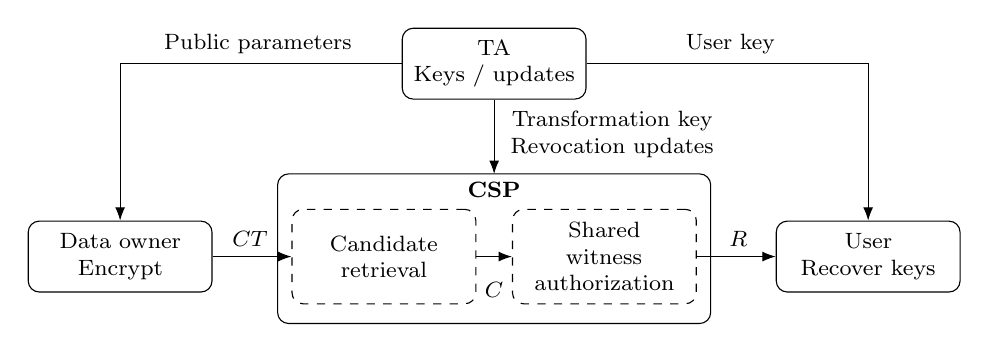
\begin{tikzpicture}[font=\footnotesize,>=Latex,
entity/.style={draw,rounded corners,align=center,minimum height=9mm,text width=21mm},
module/.style={draw,dashed,rounded corners,align=center,minimum height=12mm,text width=21mm},
lab/.style={align=center,fill=white,inner sep=1.5pt}]
\node[entity] (ta) at (0,2.45) {TA\\Keys / updates};
\node[entity] (owner) at (-4.75,0) {Data owner\\Encrypt};
\node[entity] (user) at (4.75,0) {User\\Recover keys};
\draw[rounded corners] (-2.75,-.85) rectangle (2.75,1.05);
\node[font=\footnotesize\bfseries] at (0,.85) {CSP};
\node[module] (retrieval) at (-1.4,0) {Candidate\\retrieval};
\node[module] (exec) at (1.4,0) {Shared\\witness\\authorization};
\draw[->] (ta.west)-|(owner.north);
\node[lab] at (-3,2.7) {Public parameters};
\draw[->] (ta.east)-|(user.north);
\node[lab] at (3,2.7) {User key};
\draw[->] (ta.south)--(0,1.05);
\node[lab,anchor=west] at (.15,1.55) {Transformation key\\Revocation updates};
\draw[->] (owner.east)--(retrieval.west);
\node[lab] at (-3.1,.22) {$CT$};
\draw[->] (retrieval.east)--(exec.west);
\node[lab] at (0,-.42) {$C$};
\draw[->] (exec.east)--(user.west);
\node[lab] at (3.1,.22) {$R$};
\end{tikzpicture}
\caption{Four roles, with retrieval and authorization inside one CSP.
$CT$ denotes uploaded ciphertexts and $R$ the authorized target transforms.
The measured retrieval component is a controlled candidate lookup stub,
not encrypted EII search.}
\label{fig:system}
\end{figure}

\begin{figure}[!htbp]
\centering
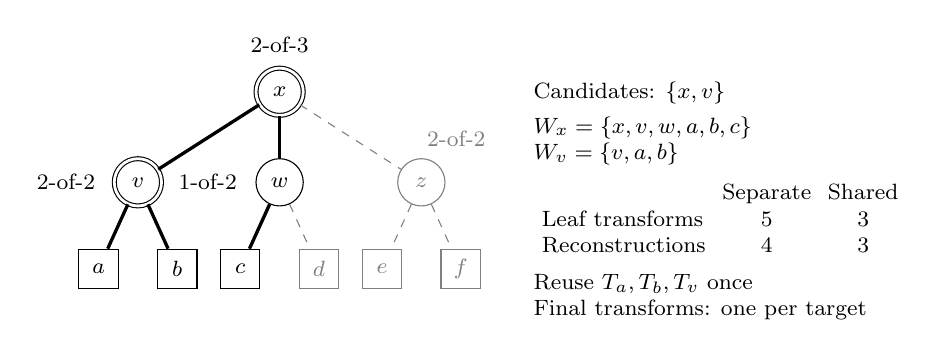
\begin{tikzpicture}[font=\footnotesize,
gate/.style={draw,circle,minimum size=6mm,inner sep=0pt},
leaf/.style={draw,rectangle,minimum size=5mm,inner sep=0pt},
target/.style={double,double distance=1pt},
unused/.style={draw=gray,text=gray},
sel/.style={very thick},other/.style={dashed,gray}]
\node[gate,target] (x) at (-2.4,2.4) {$x$};
\node[gate,target] (v) at (-4.2,1.25) {$v$};
\node[gate] (w) at (-2.4,1.25) {$w$};
\node[gate,unused] (z) at (-.6,1.25) {$z$};
\node[leaf] (a) at (-4.7,.15) {$a$};
\node[leaf] (b) at (-3.7,.15) {$b$};
\node[leaf] (c) at (-2.9,.15) {$c$};
\node[leaf,unused] (d) at (-1.9,.15) {$d$};
\node[leaf,unused] (e) at (-1.1,.15) {$e$};
\node[leaf,unused] (f) at (-.1,.15) {$f$};
\draw[sel] (x)--(v);\draw[sel] (x)--(w);\draw[other] (x)--(z);
\draw[sel] (v)--(a);\draw[sel] (v)--(b);
\draw[sel] (w)--(c);\draw[other] (w)--(d);
\draw[other] (z)--(e);\draw[other] (z)--(f);
\node[above=2pt] at (x.north) {2-of-3};
\node[anchor=east] at (-4.62,1.25) {2-of-2};
\node[anchor=east] at (-2.82,1.25) {1-of-2};
\node[anchor=west,text=gray] at (-.65,1.8) {2-of-2};
\node[align=left,anchor=north west] at (.7,2.65) {
Candidates: $\{x,v\}$\\[3pt]
$W_x=\{x,v,w,a,b,c\}$\\
$W_v=\{v,a,b\}$\\[5pt]
{\setlength{\tabcolsep}{3pt}\begin{tabular}{lcc}
 & Separate & Shared\\
Leaf transforms & 5 & 3\\
Reconstructions & 4 & 3
\end{tabular}}\\[4pt]
Reuse $T_a,T_b,T_v$ once\\
Final transforms: one per target};
\end{tikzpicture}
\caption{Ten-node example: candidates $x,v$ (double circles), all leaves
eligible. Minimum-leaf choices use ties $v<z$, $c<d$. Dashed paths are
unselected, not unauthorized; counts illustrate operations, not latency.}
\label{fig:worked}
\end{figure}
\end{revision}

\section{Attribute-Only Hierarchical Construction}
\begin{revision}
\label{sec:construction}
Our Type-3 base evaluator combines established threshold sharing,
hierarchical policies, outsourcing, and user-tree
covers~\cite{Shamir1979SecretSharing,Wang2016FileHierarchy,Green2011OutsourcedABE,Naor2001Cover}.
Figure~\ref{fig:worked} illustrates its file nodes and attribute leaves.
Our contribution is shared execution (Section~5), not a new security
reduction. User identifiers locate cover paths; they provide neither tracing
nor global user revocation.


\paragraph{Setup and KeyGen.}
Let $e:G_1\times G_2\to G_T$ have prime order $p$, generators $g_1,g_2$,
and $Z=e(g_1,g_2)$. Use $H:\{0,1\}^*\to G_1$ (hash-to-curve),
$H_2:G_1\to\mathbb F_p^*$, and a KDF. RFC~9380 specifies hash-to-curve
methods~\cite{FazHernandez2023HashToCurve}. The authority samples nonzero
$\alpha,\beta_1,\beta_2,\theta,t_i,v_j$, with $i$ an attribute and $j$ a
node in the user binary tree $BT$. Public parameters include
$f_1=g_2^{\beta_1}$, $f_2=g_2^{\beta_2}$, $Z^\alpha$, $g_1^\theta$, and
$B_i=g_1^{v_{\rm root}/t_i}$; their exponents remain secret.
For user $u$ with attributes $S_u$, choose nonzero $r_u,\tau_u,r_{i,u}$.
The cloud transformation key contains
\begin{align}
 D_1&=g_1^{\tau_u(\alpha+r_u)/\beta_1},&
 D_2&=g_1^{\tau_u r_u/\beta_2},\nonumber\\
 K_i&=(g_1^{r_u}H(i)^{r_{i,u}})^{\tau_u},&
 L_i&=g_2^{\tau_u r_{i,u}},\label{eq:keys}\\
 E_{i,j}&=g_2^{\tau_u t_i r_{i,u}/v_j}
 &&(i\in S_u,\ j\in path(u)).\nonumber
\end{align}
The user keeps $\tau_u$ private, so the cloud receives only blinded
components and leaves final unblinding to the user.

\paragraph{Encrypt.}
Sibling indices are distinct nonzero elements of $\mathbb F_p$.
Use polynomial threshold sharing~\cite{Shamir1979SecretSharing}:
for each internal node $x$, choose a degree-$(k_x-1)$ polynomial $q_x$.
At the root $r$, set $q_r(0)=\sigma_r$. At every non-root internal node, set
$q_x(0)=q_{parent(x)}(index(x))=\sigma_x$. The leaf share is
$s_y=q_{parent(y)}(index(y))$;
write $s_x=\sigma_x$ for internal nodes. Each internal file has independent
noise $z_x=\epsilon_x$ and key $ck_x\in G_T$. Choose $r_d\ne0$, publish
$A=g_1^{r_d}$, and set $\rho=H_2((g_1^\theta)^{r_d})$, $k_{i,0}=\rho$.
The authority can recover $\rho=H_2(A^\theta)$. Initially all attribute
revocation sets are empty. The general epoch-$b$ representation is
\begin{align}
 C_{1,x}&=ck_xZ^{\alpha(s_x+z_x)},& C_{2,x}&=f_1^{s_x+z_x},& C_{3,x}&=f_2^{z_x},\label{eq:files}\\
 A_y&=g_2^{s_y},& B_y&=H(i)^{s_y}g_1^{k_{i,b}},\nonumber\\
 F_{i,j,b}&=g_1^{k_{i,b}v_j/t_i},j\in Y_{i,b}.\label{eq:leaves}
\end{align}
Here $i=att(y)$ and $Y_{i,b}=KUNode(BT,ARL_{i,b})$ is the set of maximal
user-tree subtrees containing no revoked leaf. Their descendant leaves cover
exactly the users not revoked for attribute $i$. At epoch zero the
owner computes the root header as $B_i^\rho$. Encrypt each payload using
$\mathrm{KDF}(ck_x)$ and authenticated symmetric encryption. Ciphertexts,
headers, and updates are bound to their tree/version; $k_{i,b}$ is tree-local.

\paragraph{Attribute update and ReEncrypt.}
For each changed attribute, extend $ARL_i$, select a fresh mask different from
$k_{i,b-1}$, and replace its cover/header in~\eqref{eq:leaves}. Unchanged
attributes retain both their masks and headers. Generate degree-$(k_x-1)$
drift polynomials $d_x$ top-down: $d_r(0)=\eta_r$ and
$d_x(0)=\eta_x=d_{parent(x)}(index(x))$; define leaf drifts likewise.
The authority issues $(Z^{\alpha\eta_x},f_1^{\eta_x})$ per
internal node and $(g_2^{\eta_y},H(i)^{\eta_y}g_1^{\Delta k_i})$ per leaf,
where $\Delta k_i=k_{i,b}-k_{i,b-1}$. The cloud samples independent $\delta_x$
and multiplies the current components by
\begin{align}
 C_{1,x}:&\ Z^{\alpha\eta_x}(Z^\alpha)^{\delta_x},&
 C_{2,x}:&\ f_1^{\eta_x}f_1^{\delta_x},&
 C_{3,x}:&\ f_2^{\delta_x},\label{eq:update}\\
 A_y:&\ g_2^{\eta_y},& B_y:&\ H(i)^{\eta_y}g_1^{\Delta k_i}.\nonumber
\end{align}
These multipliers implement $s_v\leftarrow s_v+\eta_v$ and
$z_x\leftarrow z_x+\delta_x$, preserving~\eqref{eq:files}--\eqref{eq:leaves};
$q_x\leftarrow q_x+d_x$ preserves the threshold relations. Payloads and keys
remain unchanged. Atomic snapshot publication invalidates old query caches,
restricting subsequent authorization without retracting previously obtained
keys or plaintexts.

\paragraph{Transform and Recover.}
An eligible leaf must have $i\in S_u$ and a cover node
$j\in path(u)\cap Y_{i,b}$. Otherwise it returns $\bot$. With that node,
\begin{equation}
 T_y=\frac{e(K_i,A_y)\,e(F_{i,j,b},E_{i,j})}{e(B_y,L_i)}
     =Z^{\tau_u r_u s_y}.\label{eq:leafcancel}
\end{equation}
For any $k_x$ valid children $S_x$, let $I_x=\{index(v):v\in S_x\}$.
With $\Delta_{i,I}(0)=\prod_{j\in I\setminus\{i\}}(-j)/(i-j)$, interpolation gives
$T_x=\prod_{v\in S_x}T_v^{\Delta_{index(v),I_x}(0)}=Z^{\tau_u r_u s_x}$.
Each authorized target is then transformed and recovered by
\begin{equation}
 R_x=\frac{e(D_1,C_{2,x})}{T_xe(D_2,C_{3,x})}
     =Z^{\tau_u\alpha(s_x+z_x)},\qquad
 ck_x=C_{1,x}/R_x^{1/\tau_u}.\label{eq:recover}
\end{equation}
The attribute-header pairing in~\eqref{eq:leafcancel} is reusable for the same
user, attribute, cover, key, and epoch. The other two leaf pairings require
identical leaf operands; two final pairings remain per authorized target.
\end{revision}

\section{Shared-Witness Authorization}
\begin{revision}
\subsection{Witness Selection and Baselines}
Both selective executors choose $W_x=\Witness(x,\PolicyState)$ by the same
minimum-leaf dynamic program. Eligible leaves have $L(v)=1$, others
$L(v)=\infty$. At threshold $k_v$, select the first $k_v$ satisfiable children
sorted by $(L(c),\mathit{nodeID}(c))$, or set $L(v)=\infty$ if too few exist.
For the selected set $A_v$,
\[
 L(v)=\sum_{c\in A_v}L(c),\qquad |A_v|=k_v.
\]
Disjoint subtrees make leaf counts additive, establishing minimality by
induction; labels, weighted cost, and cross-target union size are not
minimized. Node-ID ties ensure consistent choices; merging rejects conflicts.

FullTree evaluates the whole tree and projects onto $C$. PerTarget-MinWitness
evaluates witnesses independently; Cached-UnionWitness evaluates
\[
 W_{\cup}=\bigcup_{x\in C}W_x
\]
over exact operation identities. Both can cache attribute headers equally;
sharing full leaf/reconstruction results is a separate optimization. Equal
labels with different shares remain distinct. Section~7 defines timing switches.

\subsection{Execution and Cache Validity}
The executor normalizes candidates, pins the state, and merges operations only
when their operands, selected children, and coefficients match. Header-pairing
entries bind the actual operands to
\[
\begin{split}
(&\mathit{treeID},u,a,\mathit{coverNode},b,\mathit{tkID},\\
 &\mathit{ciphertextVersion},\mathit{accessTreeHash}).
\end{split}
\]
The resulting graph is evaluated in dependency order, followed by each
authorized target's final transform. Unsatisfied targets fail, and caches
are discarded after the call, including between timing repetitions.

\subsection{Execution Procedure and Cost}
Algorithm~\ref{alg:shared} returns cloud transforms for user recovery.
In Fig.~\ref{fig:worked}, reusing $T_a,T_b,T_v$ reduces leaf transforms from
five to three and reconstructions from four to three. Same-branch placement
alone is insufficient: an ancestor witness must include the descendant;
non-ancestral target subtrees are disjoint.

\paragraph{When reuse is unavailable.}
Sharing is unavailable for disjoint witnesses, independently encrypted
policies, or equal attribute labels attached to different leaf operands.
Ancestor--descendant candidates also share no work when the selected
ancestor witness excludes the descendant. Results bound to different users,
keys, or ciphertext/update versions cannot be merged. Attribute-header
caching may still help when complete witness nodes do not overlap, but
both main baselines already receive that benefit. With little reusable
work, merging overhead can erase the latency savings; each target's final
transform and recovery remain separate.
\begin{algorithm}[!htbp]
\ifmarkrevisions\color{RevisionBlue}\fi
\caption{Shared-witness authorization for one query}
\label{alg:shared}
\begin{algorithmic}[1]
\Require Candidates $C$, pinned state $\PolicyState$, cloud key $TK_u$
\Ensure Authorized identifier-to-transform mapping $O$
\State $A,O,\mathcal H,V\gets\varnothing$
\For{$x\in\mathsf{Unique}(C)$}
  \State $W_x\gets\Witness(x,\PolicyState)$
  \If{$W_x\ne\bot$} \State $A\gets A\cup\{x\}$ \EndIf
\EndFor
\State $G\gets\mathsf{Merge}(\{W_x:x\in A\})$ using exact identities
\For{$v$ in bottom-up order of $G$}
  \If{$v$ is a leaf}
    \State $h\gets\mathsf{HeaderBinding}(v,\PolicyState,TK_u)$
    \State $\mathcal H[h]\gets\mathsf{HeaderPairing}(v,TK_u)$ if absent
    \State $V[v]\gets\mathsf{LeafTransform}(v,\mathcal H[h])$
  \Else \State $V[v]\gets\mathsf{Interpolate}(\{V[c]\},I_v)$ \EndIf
\EndFor
\State $O\gets\{fid_x\mapsto\mathsf{Finalize}(x,V[x]):x\in A\}$
\State Discard $\mathcal H,V$; \Return $O$
\end{algorithmic}
\end{algorithm}

Let $L_\Sigma,I_\Sigma$ count leaf and reconstruction occurrences in separate
witnesses, and $L_\cup,I_\cup$ their unique reusable operations. With equal
header caching, sharing avoids $2(L_\Sigma-L_\cup)$ leaf-specific pairings
and $I_\Sigma-I_\cup$ reconstructions, whose costs depend on selected children.
Two final pairings per authorized target and user recovery remain; saved work
must outweigh merging and cache management.

\paragraph{Observed witness overlap.}
Measured overlap $\omega=1-|W_\cup|/\sum_x|W_x|$ counts repeated leaf and
internal occurrences, not matching labels. Leaf reduction $1-L_\cup/L_\Sigma$
counts only leaves, explaining the related but distinct panels of
Fig.~\ref{fig:v2overlap}. Neither quantity is a preset level or latency predictor.
\end{revision}

\section{Correctness, Revocation, and Security Boundaries}
\begin{revision}
\subsection{Conditional Execution Equivalence}
\noindent\textbf{Proposition.}
If the base evaluator is correct on $\PolicyState$, witness selection is sound
and complete for supported policies, and cache identities bind identical
inputs and state, then user recovery gives
\[
 \Result_{\CU}(C,\PolicyState)=\Result_{\PT}(C,\PolicyState)
                  =\left.\Result_{\FT}(\PolicyState)\right|_C.
\]
\noindent\emph{Argument.}
Identical leaf operands yield identical values. Inductively, every merged
reconstruction receives the same children and coefficients as independent
execution. Final transforms and recovery are unchanged, while sound and
complete selection preserves the target set. Base correctness gives equality
with FullTree's candidate projection, and normalization preserves identifiers.

\subsection{Algebraic Correctness and Revocation}
Bilinearity cancels the $H(i)$ terms in~\eqref{eq:leafcancel}; the header term
$e(F_{i,j,b},E_{i,j})=Z^{\tau_u r_{i,u}k_{i,b}}$ cancels the mask.
Interpolation yields $T_x$, and the denominator in~\eqref{eq:recover} is
$Z^{\tau_u r_u(s_x+z_x)}$, leaving the required $\alpha$ term. The update
relations preserve this reasoning at each honest snapshot. Covers exclude
only the users revoked for the affected attribute; an all-revoked cover is
empty. Combining an old header with a new leaf leaves residual
$Z^{\tau_u r_{i,u}(k_{i,b-1}-k_{i,b})}$ and is invalid for that leaf.

An independent recursive threshold oracle checks complete target sets and
recovered keys for all five executors. Its 18 properties cover nested
thresholds, repeated attributes, denial and alternative paths, cumulative
and duplicate revocations, control users, injected stale caches, wire
decoding, and role isolation. Incremental and independently reconstructed
states agree byte for byte. These are functional checks, not a security proof.

\subsection{Observable Information}
The execution exposes candidates, witnesses, failures, plans, cache hits, and
timing in addition to the index's token/access/update patterns. Policies,
labels, sizes, and revocation paths remain visible. Thus equal outputs do not
imply indistinguishable execution traces, and we claim no such protection.
\end{revision}

\section{Experimental Methodology}
\begin{revision}
\subsection{Experimental Setup and Baselines}
The frozen BLS12-381 Type-3 implementation passes functional tests before
timing. Four configurations switch witness sharing and header caching:
\begin{center}
\begin{tabular}{lcc}\toprule
Configuration & Share witness nodes & Cache attribute headers\\\midrule
PT00 & No & No\\ PT01 & No & Yes\\
Union10 & Yes & No\\ Union11 & Yes & Yes\\\bottomrule
\end{tabular}
\end{center}
PT01/Union11 includes each method's planning with equal caching; FullTree11
checks correctness only. Discovery crosses two layouts and $|C|\in\{4,16\}$
with six seeds, five instances each (120 units). The Same-Branch, $|C|=16$
holdout has 30 units from six unused seeds. Revocation has nine four-event
sequences (three seeds per size); complete calls have nine Same-Branch,
$|C|=16$ instances.

\paragraph{Workloads and interpretation.}
Authorization policies have 100 internal file nodes arranged breadth-first,
at most four internal children plus one attribute leaf per node, and threshold
$\min(2,\text{child count})$. Attribute labels draw from 32 values through
$(7i+J_i)\bmod32$, $J_i\in\{0,1,2,3\}$, for node $i$. The user tree has 16
users; the timed user holds every occurring attribute, so main candidates are
all authorized. Functional tests cover denials, not mixed-authorization timing.
Same-Branch samples within one root-child branch; Disjoint-Branches samples
round-robin within up to four branches. The latter need not have disjoint
witnesses within a branch. A global fallback handles insufficient pools,
so measured overlap describes the realized instances.

The parameters isolate ancestor--descendant reuse rather than represent
deployment statistics. The holdout tests the same synthetic family; natural
policy and query statistics are needed to establish real overlap frequency.

\subsection{Timing and Statistics}
Authorization timing includes validation, planning, caching, and final
transforms, excluding setup, encryption, retrieval, and user recovery.
After three warmups, seven rounds use randomized method order and batches
of at least 20 ms. Any initial method CV above 5\% triggers seven additional
rounds for all methods of that instance; all are retained. With median $t_{j,i}$,
\[
 s_i=t_{\mathrm{PT01},i}/t_{\mathrm{Union11},i},\qquad
 \widetilde{s}=\mathsf{median}_i(s_i).
\]
The percentile bootstrap resamples six five-instance seed clusters 10,000
times (RNG seed 20260917). Rounds and batch repetitions are not independent
samples~\cite{Kalibera2013Benchmarking}.

One process is pinned to logical CPU 0 on an Intel Core i7-10750H with
15.84 GiB RAM, Windows 11 build 10.0.26200, CPython 3.14.6,
\texttt{chia\_rs} 0.49.0, and \texttt{py-ecc} 8.0.0. We use
\texttt{perf\_counter\_ns} and default garbage collection. Complete calls
include a dictionary candidate lookup, not encrypted EII processing.

\paragraph{Implementation correspondence and reproducibility.}
The backend retains auxiliary $g_2^{s_x+z_x}$ alongside $C_1,C_2,C_3$.
Although Recover does not use it, its construction, update costs, and bytes
remain measured; a three-component format was not remeasured. The local
artifact includes source, raw, frozen protocol/hashes, tests, and plotting
scripts. Its wrapper checks correctness and reanalyzes raw without timing;
public hosting remains pending.
\end{revision}

\section{Results}
\begin{revision}
\subsection{Authorization Speedup and Holdout}
The strongest replicated gain is for 16 same-branch targets
(Fig.~\ref{fig:v2speedup}): $1.163\times$ discovery and $1.159\times$ holdout,
or 14.0\% and 13.7\% lower authorization time. Larger same-branch sets offer
more ancestor--descendant reuse (Fig.~\ref{fig:worked}); four targets or
cross-branch placement expose less shared work. Gains depend on selected
witnesses, not layout alone.

\begin{figure}[!htbp]
\centering
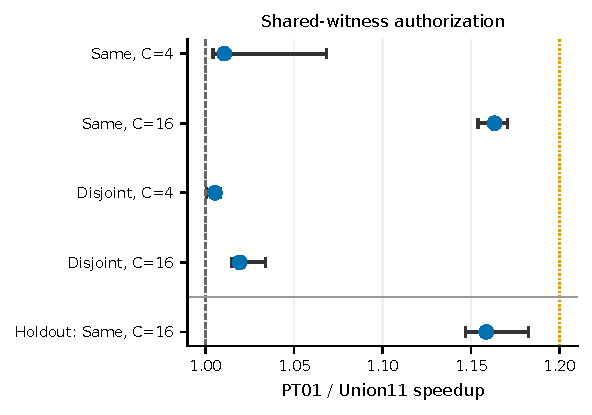
\includegraphics[width=.72\linewidth]{figures/fig1_primary_speedup.pdf}
\caption{PT01/Union11 authorization speedup: medians of 30 instance ratios per
configuration, with 95\% percentile seed-cluster bootstrap intervals over
six five-instance clusters. The fresh-seed holdout is separated.}
\label{fig:v2speedup}
\end{figure}

\subsection{Mechanism and Ablation}
Same-Branch, $|C|=16$ reduces median leaf transforms by 26.3\%, interpolations
by 26.0\%, and pairings by 13.0\% (Fig.~\ref{fig:v2overlap}). Node overlap and
leaf savings have different denominators. Remaining final transforms and
planning prevent proportional latency gains; the association supports reuse
without proving causality.

\begin{figure}[!htbp]
\centering
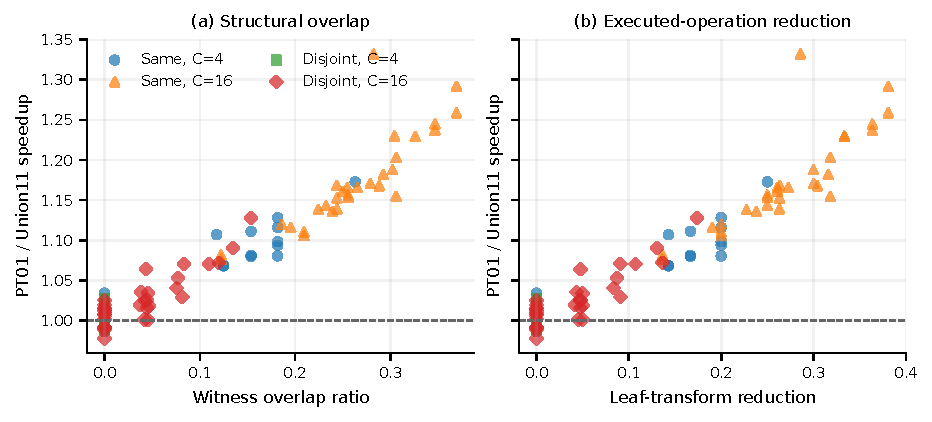
\includegraphics[width=\linewidth]{figures/fig2_overlap_reuse.pdf}
\caption{Each point is one of 120 discovery instances on a 100-internal-node tree.
Layout and $|C|$ are controlled; overlap and leaf reduction are observed
per-instance values. Both panels use its PT01/Union11 ratio; the line marks
no speedup.}
\label{fig:v2overlap}
\end{figure}

PT00 normalization in Fig.~\ref{fig:v2ablation} separates caching, sharing,
and their combination. Sharing alone already lowers Union10's median latency
for Same-Branch, $|C|=16$. Median ratios to Union11 are 1.218 (PT00), 1.163
(PT01), and 1.026 (Union10): only PT01/Union11 isolates sharing with equal
caching. Some instances favor Union10, potentially because cache management
adds work, merging reduces header-hit opportunities, or noise reverses close
rankings. These contributions were not isolated; caching is not shown to be
intrinsically harmful.

\begin{figure}[!htbp]
\centering
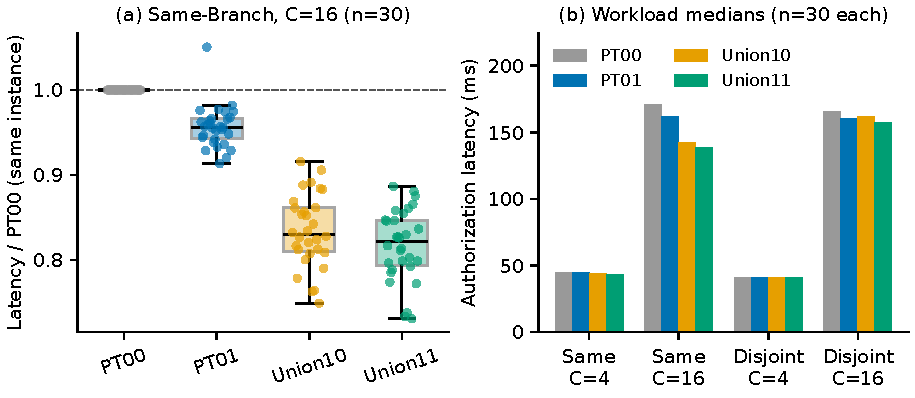
\includegraphics[width=\linewidth]{figures/fig3_ablation.pdf}
\caption{(a) Same-Branch, $|C|=16$: instance-median latency divided by the same
instance's PT00 latency ($n=30$); lower is faster. Boxes show quartiles,
whiskers cover observations within 1.5 IQR, and dots show all instances.
(b) Absolute medians for four configurations ($n=30$ each).}
\label{fig:v2ablation}
\end{figure}

\subsection{Controlled Complete Call}
User recovery limits complete-call gains (Fig.~\ref{fig:v2e2e}). Nine
instances yield total medians of 168.97/152.70 ms for PT01/Union11 and a
median instance ratio of $1.091\times$ (8.4\% lower time), distinct from the
ratio of aggregate medians. Stage means are additive within recorded rounds.
The call ends at key recovery, excluding transfer and bulk decryption;
the lookup stub does not measure encrypted EII.

\begin{figure}[!htbp]
\centering
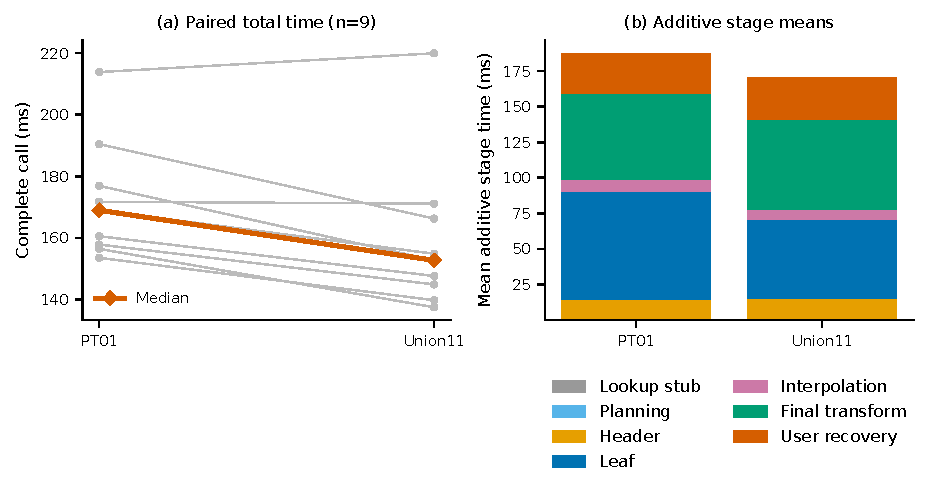
\includegraphics[width=\linewidth]{figures/fig4_end_to_end.pdf}
\caption{Nine Same-Branch, $|C|=16$ instances on 100-node policies (three seeds,
three instances each): (a) paired total medians; (b) additive stage means.
Both methods cache headers equally. Timing ends at file-key recovery;
candidate lookup is an in-memory stub.}
\label{fig:v2e2e}
\end{figure}

\subsection{Revocation Cost and Correctness}
Nine sequences (36 updates) preserve complete target sets and keys,
including the control user's access; incremental states match independent
reconstructions. At 25/100/250 nodes, median TA/CSP times are 143.9/142.9,
571.9/575.5, and 1450.1/1425.1 ms. Canonical streams occupy 23.3/92.1/229.8
KiB, including bindings, covers, and framing (Fig.~\ref{fig:v2revocation}).
These observations do not establish asymptotic complexity.

\begin{figure}[!htbp]
\centering
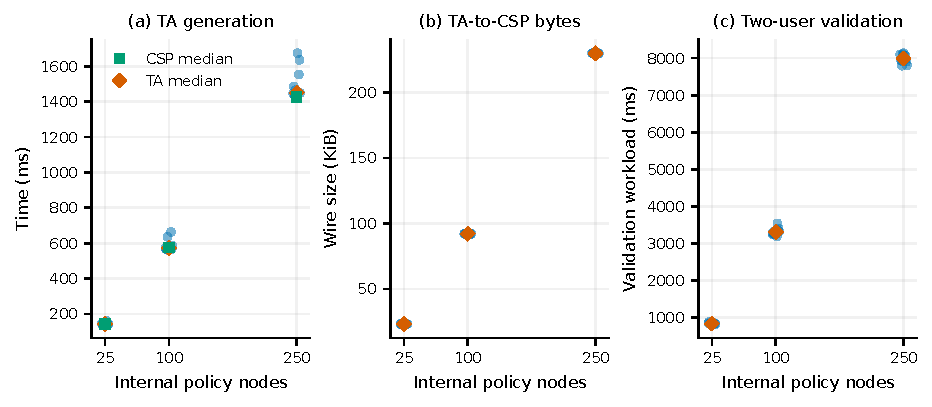
\includegraphics[width=\linewidth]{figures/fig5_revocation.pdf}
\caption{Nine four-event sequences, three seeds per size (25, 100, 250 internal
nodes): (a) TA generation and CSP decode/generation/application; (b) actual
TA-to-CSP bytes, including the retained auxiliary component; (c) two-user,
all-target post-update validation, not per-query authorization latency.}
\label{fig:v2revocation}
\end{figure}

\subsection{Measurement Stability and Timing Variability}
\label{sec:stability}
The 5\% CV rule triggered supplementation in 74/120 discovery, 6/30 holdout,
and 8/9 complete-call instances. Final CV exceeds 5\% for 148/480, 5/60,
and 15/18 instance--method combinations, respectively (Fig.~\ref{fig:v2stability}).
Median CVs are 3.5\%, 2.5\%, and 16.0\%; complete calls are substantially
noisier. All observations remain. Extra rounds ensure neither convergence
nor absence of bias, and the variation sources were not isolated.

\begin{figure}[!htbp]
\centering
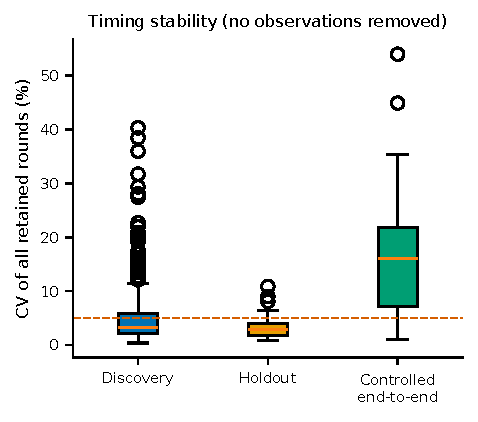
\includegraphics[width=.72\linewidth]{figures/fig6_timing_stability.pdf}
\caption{CV over all retained rounds: 480 discovery, 60 holdout, and 18 complete-call
instance--method combinations. Discovery covers four configurations; holdout
and complete calls use Same-Branch, $|C|=16$. The line is the initial-block
5\% trigger; no high-CV observations are removed.}
\label{fig:v2stability}
\end{figure}
\end{revision}

\section{Limitations and Conclusion}

\begin{revision}
Shared-witness execution preserves independent results under the stated
assumptions and yields $1.163\times$ discovery/$1.159\times$ holdout speedups
for 16 same-branch targets with equal caching. Per-target transforms and
recovery limit complete-call gains. Synthetic, fully authorized, fixed-size
workloads leave natural overlap, scaling, and mixed authorization unresolved.
Complete calls use a lookup stub and show high variability; revocation excludes regrant, tree
growth, new trees after revocation, and rollback protection. Functional and
role checks prove neither IND-CPA nor collusion resistance.
\end{revision}

\subsubsection*{Acknowledgements}
This work was supported by the Postgraduate Research \& Practice Innovation Program of Jiangsu Province under Grant No.~26CXJH1216.

\clearpage
% Count all body pages, including floats flushed by clearpage.
\phantomsection\label{page:referencesstart}
\IfFileExists{splncs04.bst}{\bibliographystyle{splncs04}}{\bibliographystyle{plain}}
\bibliography{references}
\end{document} 
